\chapter{Análisis y diseño}
\section{Análisis previo}
Durante esta sección se analizarán cuestiones importantes que afectarán a múltiples secciones posteriores y que es necesario plantearse antes de comenzar, ya que pueden afectar de manera muy significativa a la elección y posterior diseño de futuros apartados.

De manera general, se deben tener en cuenta los siguientes factores:
\begin{itemize}
    \item El tipo de datos que se van a guardar.
    \item El tipo y la cantidad relaciones entre los datos.
    \item La forma de identificar los datos. 
    \item La forma de mostrar los datos. 
    \item Cómo se va a buscar información y qué búsquedas se van a realizar.
    \item La cantidad de información que se va a almacenar. 
\end{itemize}

\subsection{Tipos de datos}
Dentro de los tipos de datos se tienen que distinguir dos tipos, por un lado, están los mensajes que el usuario envía y por otro los datos que se extraen de ellos. 
\subsubsection{Tipos de datos a analizar}\label{diseno:tipo_dato}
Dentro de los mensajes, este proyecto se centrará en mensajes de correo electrónico, por lo que hay fundamentalmente de tres tipos de datos, en texto plano, en HyperText Markup Language (HTML) \cite{html_wiki} y en formato (EML).

A la hora de elegir un lenguaje, contar con alguna librería que sea capaz de analizar dichos tipos de archivos es algo crítico, puesto que hacer un analizador de dichos tipos sería muy costoso y llevaría demasiado tiempo. Mientras la mayoría de los lenguajes modernos tienen librarías para leer archivos en HTML, no ocurre los mismo para el formato EML. 

Sin embargo, el diseño no debe limitar la implementación de otros tipos de archivos tales como comma-separated values (CSV), Extensible Markup Language (XML) o JavaScript Object Notation (JSON). 

\subsubsection{Tipos de datos que se van a extraer}
En un principio los datos que se van a extraer son enlaces, dominios, direcciones de correo, direcciones de Internet Protocol (IP) y en el caso de los archivos en formato EML, sus cabeceras. 

\subsection{Tipo y cantidad de relaciones}
El tipo de relaciones serán normalmente de muchos a muchos, ya que de un único mensaje se pueden extraer varios datos de un mismo tipo, que a vez pueden estar múltiples mensajes.

Respecto a la cantidad de relaciones, mientras que de un correo no se deben extraer demasiados datos, un dato concreto puede aparecer en una gran cantidad de correos, por lo que en función del diseño que se haga, recuperar todos los correos en los que aparece un determinado dato podría llegar a ser una operación muy costosa. 

\subsection{Forma de identificar los datos} \label{diseno:identificar_datos}
En este proyecto y debido a la naturaleza de los datos que se tratan, algo que pudiera ser trivial como es el hecho de identificar un dato concreto, se vuelve una tarea más compleja, pues estos pueden ser relativamente grandes y no se deben tratar de la misma manera que otros de menor tamaño, como tal vez puede ser un número o una fecha. 

También es importante el hecho de poder “navegar” mediante enlaces, ya que no tendría sentido poner como dirección de un mensaje su propio contenido.

Este problema se puede solucionar de múltiples formas, una de ellas, consistiría en asignar a cada dato un valor numérico e incremental, de modo que se podría acceder al dato número 1, 2, …, n. Este sistema permite tener un control del número de elementos que se han analizado, además ocupa muy poco (con 4 bytes por elemento se podrían numerar 4.294.967.296 elementos de dicho tipo), permitiría hacer búsquedas rápidas, al poder guardar en memoria una gran cantidad de elementos y no guarda relación alguna con el elemento al que identifica.

Sin embargo, también presenta los siguientes problemas, y es que, al no guardar relación con el elemento, no se puede obtener el identificador únicamente con el valor del dato, por lo que requiere de una consulta del valor completo a la base de datos, que, en el caso de un mensaje, puede ser de gran tamaño.

Para evitar esta falta de relación entre el valor de un elemento y su identificación se puede utilizar una función hash, que sea rápida y que devuelva valores pequeños. Esto solucionaría la falta de correlación entre identificador y valor, facilitaría la navegación, permitiría búsquedas rápidas, (Constantes en teoría) y simplificaría las búsquedas de datos grandes como los mensajes.

Aunque también presenta problemas, el mayor de ellos es que ocupa mucho más espacio que una identificación numérica, lo que, en un sistema relacional, puede hacer que las uniones de tablas sean mucho más lentas. Además, también se pierde el orden de inserción, pero tampoco es importante en este caso.

Por tanto, una solución interesante puede ser adoptar ambos modelos, por un lado, tener un índice numérico e incremental y por otro un índice de tipo hash para buscar en caso de no tener el identificador numérico. Por ejemplo, para comprobar si un mensaje ya ha sido o no analizado se podría utilizar su hash, mientras que para las uniones de tablas de podría utilizar el identificador numérico. 

Esta solución también presenta el problema de sobrecoste que conlleva guardar el hash y que puede ser mayor o menor en función de los bits que ocupe la función elegida.

Para ello, ha hecho un pequeño estudio del sobrecoste generado por cada millón de elementos insertados según algunas de las funciones hash más conocidas en este momento. No se va a tener en cuenta el coste computacional de dicha función al considerarlo relativamente bajo en todas ellas. 

También se va a considerar la probabilidad de colisiones suponiendo que todos los valores son equiprobables. Para hacer este cálculo y teniendo en cuenta la paradoja del cumpleaños, se va a calcular la probabilidad de colisiones mediante la siguiente fórmula \(k=\sqrt{2^n}\) siendo n el tamaño del hash en bits y k la probabilidad de que haya una colisión.

\begin{table}[htbp]
    \begin{center}
        \begin{tabular}{| m{1.5cm} || m{2.3cm} | m{3cm} | m{3.8cm} |}
            \hline
            Función hash	& Tamaño del hash (Bytes) & Probabilidad de colisión &	Sobrecoste generado (Por cada millón) MB \\ 
            \hline \hline 
             & & &\\  [0.03cm]
            MD5	    & 16	& \(1.84467\times10^{19}\)	    & 15.25879 \\  [0.3cm]
            SHA1	& 20	& \(1.20893\times10^{24}\)	& 19.07349 \\ [0.3cm]
            SHA256	& 32	& \(3.40282\times10^{38}\)	& 30.51758 \\ [0.3cm]
            SHA512	& 64	& \(1.15792  \times10^{77}	 \)    & 61.03516 \\ [0.3cm]
            \hline
        \end{tabular}
    \caption{Comparativa de las distintas funciones hash}
    \label{table:funciones_hash}
    \end{center}
\end{table}

En base a la tabla \ref{table:funciones_hash}, puede verse que el sobrecoste por cada millón de documentos es completamente asumible en todos los casos, pues incluso con 10 millones de elementos, en el peor de los casos, es decir usando la función SHA512, los hashes tendrían un coste de tan solo 610MB, lo que no es algo exagerado teniendo en cuenta la cantidad de elementos que se tendrían y las ventajas que se obtienen. 

Sin embargo, y dado que el hash se va a utilizar únicamente como identificador, es mucho más interesante usar una función que genere un hash de menor tamaño como podría ser MD5 o SHA1 ya que el tamaño es similar. 

Finalmente se va a optar por SHA1 debido a que MD5 en la actualidad está roto, y aunque esto no debería afectar directamente al servicio, pues no se pretender obtener ningún tipo de seguridad, sí que se podría aprovechar esta vulnerabilidad por parte de algún ciberdelincuente añadiendo él mismo un mensaje falso que genere el mismo hash que un posible correo malicioso enviado por el mismo ciberdelincuente, evitando de esta manera que sea analizado en la plataforma. 

A la hora de la elección de un lenguaje de programación, será necesario que este cuente con dicha función o en su defecto, que haya alguna implementación de esta ya desarrollada, pues no es objetivo de este trabajo desarrollarla.

\subsection{Forma de mostrar los datos} \label{diseno:datos}
La forma de mostrar los datos puede indicar o al menos sugerir de qué manera se deben almacenar para facilitar su posterior visualización.

Dependiendo del tipo de dato se puede mostrar una información u otra, aunque hay información común a todos los datos.

A continuación, se va a indicar la información común a todos los elementos y la asociada a cada uno de ellos. 


\subsubsection{Información común a todos los elementos}
La información siguiente la tendrán todos los elementos visualizados en la plataforma, sean o no mensajes. 
\begin{itemize}
    \item Valor del elemento.
    \item Hash: Es el hash del valor del elemento. 
    \item Fuente(s): Indica de dónde se ha obtenido el dato, puede ser la persona que publicó el mensaje o en caso de un enlace, la fuente podría ser un mensaje. 
    \item Tipo: Será un array con distintos posibles valores donde los usuarios podrán votar el cuál de esos tipos es.  
    \item Fecha de análisis: indica cuándo se analizó el mensaje. 
    \item Score: indica la maliciosidad del elemento, pudiendo ser fiable o malicioso
\end{itemize}

También es importante indicar que en la visualización de cualquier dato extraído de un mensaje será importante que, además de la información relacionada con el mismo (Valor, fecha de análisis, score, …), se puedan listar todos los mensajes en donde ha aparecido dicho dato, así como un enlace a cada uno de ellos. El texto mostrado en este caso será el hash del mensaje.

El poder listar los mensajes donde aparece un dato concreto es importante para poder llevar a cabo investigaciones, o identificar nuevos mensajes perniciosos en base a elementos comunes con otros mensajes ya analizados.

\subsubsection{Mensajes}
La información siguiente es específica de los mensajes.
\begin{itemize}
    \item Formato: texto plano, HTML o EML (En el futuro podría haber más como CSV, JSON, XML, …)
    \item Tipo: SPAM comercial, una estafa, una sextorsión o un ataque de phishing entre otros. 
    \item Lenguaje: indica el lenguaje del mensaje (inglés, español, francés, …)
\end{itemize}

\subsubsection{Direcciones IP}
La información siguiente es específica de las direcciones IP.
\begin{itemize}
    \item Versión: Indicara si las direcciones es IPv4 o IPv6.
\end{itemize}

\subsubsection{Dominios}
La información siguiente es específica de los dominios.
\begin{itemize}
    \item Dominio: en caso de ser un subdominio, indicará el dominio al que pertenece. 
    \item Subdominio: en caso de ser un dominio, se    indicarán todos los subdominios analizados de dicho dominio.
    \item Tipo: Legítimo, phishing. 
\end{itemize}

\subsubsection{Enlaces}
La información siguiente es específica de los enlaces.
\begin{itemize}
    \item Domino: Se indicará el dominio o el subdominio al que pertenece.
    \item Tipo: Legítimo, phishing. 
\end{itemize}

\subsubsection{Direcciones de correo electrónico}
La información siguiente es específica de las direcciones de correo electrónico.
\begin{itemize}
    \item Domino: Se indicará el dominio o el subdominio al que pertenece.
    \item Tipo: Legítimo, phishing. 
\end{itemize}


\subsection{Cómo se va a buscar información y qué búsquedas se van a realizar} \label{diseno:busquedas}
Saber qué búsquedas van a hacer y con qué datos se cuenta para llevarlas a cabo es necesario para determinar por un lado cómo se guarda la información y, por otro lado, las relaciones necesarias para que se puedan realizar las dichas consultas.

En este caso, dado un documento se debe poder obtener a cada uno de los datos extraídos de él y dado un dato cualquiera, tienen que poder obtenerse tanto los correos en los que aparece, como otros elementos relacionados con él. Por ejemplo, dado un domino, además de los mensajes donde está presente, también se debe obtener información sobre todos los enlaces analizados pertenecientes a dicho dominio.

Las búsquedas generalmente serán de elementos concretos, es decir, no será común realizar búsquedas por rango. Tampoco será común usar los operadores de mayor o menor.

Se debe poder buscar un elemento tanto por su valor, o por su hash en caso de ser un elemento de gran tamaño, así como por su identificador numérico, ya que su búsqueda puede ser mucho más rápida. 

En un principio no será habitual buscar elementos por información relativa a ellos, por ejemplo, elementos analizados en una determinada fecha o con una determinada característica. 

También es importante señalar que al principio las operaciones de inserción serán las más comunes y que a medida que se vaya haciendo uso del servicio, las operaciones de consulta serán las que prevalecerán. Además, es necesario que el servicio no sea demasiado lento, pues no sería práctico, por este motivo, debe prevalecer la velocidad de consulta sobre la inserción. 

\subsection{Cantidad de información que se va a almacenar}\label{diseno:cantidad_info}
Respecto a la cantidad de información a almacenar, el sistema debe estar preparado para guardar un gran volumen de información, de decenas o cientos de millones de correos electrónicos, por lo que contar con un sistema escalable es crítico.  

A la hora de realizar este informe, se cuentan con más de 8.5 millones de correos electrónicos perniciosos. 


\section{Información sobre los datos que se va a extraer} \label{info_datos}
Como ya se ha comentado con anterioridad, uno de los objetivos del proyecto es extraer distintos tipos de datos y relacionarlos con otros correos electrónicos. 

En concreto se quiere extraer: 
\begin{itemize}
    \item Direcciones IP
    \item Dominios
    \item Enlaces 
    \item Direcciones de correo electrónico
\end{itemize}

Una forma sencilla de identificar y extraer este tipo de datos relativamente bien definidos es mediante expresiones regulares. El hacerlo de esta manera requiere que se sepa de manera muy precisa cómo están formados, qué símbolos tienen o no, qué tamaño,…

Por este motivo, se va a hacer un análisis exhaustivo de los distintos tipos de datos que se quieren obtener, especialmente en lo que a estructura, formato, tamaño y símbolos se refiere. Sin embargo, el análisis será eminentemente práctico, sin entrar detalles técnicos que no tengan relevancia a la hora de crear una expresión regular para evitar que la longitud de la memoria crezca en exceso. 

De esta manera se podrán crear unas expresiones regulares muy precisas que generen el mínimo número de falsos negativos posibles.

\subsection{Direcciones IP}
Una dirección IP es un conjunto de números y/o letras que identifican de manera única a cada uno de los dispositivos de una red. 

Existen dos versiones, la versión 4 y la versión 6, cada una tiene un formato distinto. \cite{ipv4_v6}

\subsubsection{IP versión 4 (IPv4)}\label{subsec:ipv4}
Cuando se habla de IPv4 es importante mencionar que su formato no se ha especificado como tal en ningún RFC, quedando definido por el uso y por cómo fue descrito en otros RFCs. Con esto en mente se va a usar el RFC790 \cite{rfc790}, donde se realiza la asignación de clases de redes, a distintos grupos de direcciones IP, para definir su formato. 

Como se puede observar en dicho RFC, se podría decir que por convención una dirección IP en versión 4 está definida por un conjunto de cuatro números, separados entre sí por un punto y cuyo valor del 0 al 255. Pueden ser escritos tanto con ceros a la izquierda o sin ellos, o lo que es lo mismo, tanto el 3 como el 03, como el 003 son válidos y tienen exactamente el mismo valor. Esto hace que una misma dirección pueda ser escrita de múltiples formas, por ejemplo 192.168.0.1 podría ser escrita como 192.168.000.001 ò 192.168.00.01 ò 192.168.000.01, etc. 
 


\subsubsection{IP versión 6 (IPv6)}
La representación textual de una dirección IPv6 es muy flexible lo que hace que sea mucho más complicado crear una expresión regular para identificarlas. Su formato de definió en el RFC 4291, en la sección 2.2 \cite{rfc4291_section2_2}, aunque debido a que ciertos operadores estaban teniendo problemas por su flexibilidad, la Internet Engineering Task Force (IEFT) publicó el RFC 5952 \cite{rfc5952} con ciertas recomendaciones sobre su formato escrito para facilitar la implementación del protocolo. 

En líneas generales una dirección IP en versión 6 está representada por 8 números hexadecimales de cuatro cifras, separados entre sí por dos puntos verticales (“:”) y escritos en normalmente en minúsculas, aunque también pueden estar escritos en mayúsculas. 

A continuación, se van a comentar algunas de las posibles variaciones a la hora de representar textualmente una dirección de este tipo. 
 
\paragraph{Omitir ceros a la izquierda}
Los 0 a la izquierda pueden (o no) ser omitidos y el valor de la dirección no se altera. Por ejemplo, las siguientes direcciones, pese a estar escritas de distinta forma, tienen el mismo valor.  

      2001:db8:aaaa:bbbb:cccc:dddd:eeee:0001

      2001:db8:aaaa:bbbb:cccc:dddd:eeee:001

      2001:db8:aaaa:bbbb:cccc:dddd:eeee:01

      2001:db8:aaaa:bbbb:cccc:dddd:eeee:1

\paragraph{Contraer los ceros}
Si en una dirección uno o más números consecutivos son cero, se pueden eliminar. Esto puede hacerse una única vez.

Por ejemplo:

      2001:db8:aaaa:bbbb:0:0:0:1

      2001:db8:aaaa:bbbb::1
      
Precisamente esta característica es la que hace sea complicado analizar una dirección IP en su versión 6, ya que múltiples opciones son posibles y todas correctas.

\paragraph{Direcciones IPv4 embebidas}\label{subsec:ipv6}
Una dirección IPv6 puede tener embebida una dirección IPv4 al final de esta, que será escrita con el mismo formato de una dirección IPv4. 

Por ejemplo 

    0:0:0:0:0:0:13.1.68.3

    0:0:0:0:0:FFFF:129.144.52.38
    
Además, si se tiene en cuenta la propiedad anterior, podrían contraerse los ceros, quedado como sigue: 

    ::13.1.68.3

    ::FFFF:129.144.52.38

\subsection{Dominios}\label{subsec:Dominios}
Un dominio es una cadena de caracteres que está asociada a una o varias direcciones IP. Está regulados por un organismo internacional llamado ICANN del inglés (Internet Corporation for Assigned Names and Numbers; ICANN) \cite{icann} y su especificación viene recogida en el RFC 1035 \cite{rfc1035}

\subsubsection{Formato}
Según este RFC un dominio está formado por dos o más partes separadas entre sí por un punto <<.>>. 

Siendo el formato como sigue: 
\begin{verbatim}
    [<Subdominio>.]<nombre de dominio>.[<SLD>.]<TLD>
\end{verbatim}

Donde: 
\begin{itemize}
    \item Subdominio: Los subdominios subpartes del dominio al que preceden. Puede haber tantos como se quiera.
    \item Nombre de dominio: Se registra en el ICANN o la autoridad competente dependiendo del top-level domain (TLD) o del second-level domain (SLD).
    \item SLD: Son conocidos como dominios de segundo nivel y permiten una especificación de un dominio de primer nivel. Por ejemplo, <<co.es>> podría estar destinado a empresas comerciales españolas. Todos los SLDs registrados pueden ser consultados en Publicsuffix \cite{SLD_list}.
    \item TLD: Son conocidos como dominios de primer nivel y son los gestionados por el ICANN. Todos los TLDs registrados se pueden encontrar en la web del Internet Assigned Numbers Authority (IANA) \cite{TLD_list}
\end{itemize}

Tener en cuenta los TLDs y los SLDs es muy importante para asignar correctamente los dominios y los subdominios, ya que no tener en cuenta los SLDs podría hacer que se considerasen nombres de dominio que no lo son. 

Además, es una buena forma de detectar falsos positivos cuando se están buscando dominios en un documento de texto.

\subsubsection{Tamaño}
En la sección “2.3.4. Size limits” del RFC 1035, se indica que el tamaño máximo para el dominio son 255 completo caracteres y el de casa sección de 63 caracteres, aunque en la actualidad no suelen ser tan largos. 

\subsubsection{Caracteres permitidos} \label{subsec:caracteres_permitiros_dominios}
Así mismo en la sección “2.3.3. Character Case” se indica que la codificación de un dominio debe ser ASCII del inglés (American Standard Code for Information Interchange) e insensible a mayúsculas y minúsculas, aunque no obliga a ello. En el RFC 3490 \cite{rfc3490}, se recoge la posibilidad de usar caracteres Unicode aunque estos sean representados internamente como caracteres ASCII, en la práctica, los caracteres Unicode no son muy usados.

Además, y según se especifica en el RFC 952 \cite{rfc952} y en el RFC 1123 \cite{rfc1123}, los únicos caracteres válidos dentro de un dominio son los caracteres alfanuméricos (A-Z) y (0-9), el guion medio (-) y el punto (.), aunque algunos servidores también permiten el guion bajo (\_).

\subsection{Enlaces (URLs)} \label{subsec:Enlaces}
Los enlaces o URLs (del inglés Uniform Resource Locator) vienen definidas por el RFC 1738 \cite{rfc1738}, de especial interés la sección “3. Specific Schemes”. Una URL es a su vez un tipo de URI (del inglés Uniform Resource Identifier) definido en el RFC 3986 \cite{rfc3986}, de este último el apartado más interesante para el proyecto es la sección “3.3.  Path” en el cual se especifica el formato que debe tener y también en el “Apéndice A: Collected ABNF for URI”.

También es interesante el RFC 3696 en la sección “4.1.  URI syntax definitions and issues” \cite{rfc3696_section4_1}, ya que se centra en las URLs cuyo esquema sea Hypertext Transfer Protocol (HTTP) o HTTP seguro (HTTPS), y por tanto el más interesante para el proyecto .

\subsubsection{Formato}
El formato viene definido como sigue: 
\begin{verbatim}
    {http/https}://<dominio>[:<puerto>][/<ruta[<parámetros>]>]
\end{verbatim}

Donde:
\begin{itemize}
    \item http/https: Define el protocolo y aparecerá uno u otro. 
    \item Dominio: su formato ya ha sido definido.
    \item Puerto: No es muy usado, es un valor numérico que va del 0 al 65535.
    \item Ruta: son distintas cadenas de texto que dan acceso a cada una de las páginas de un mismo dominio.
    \item Parámetros: Son posibles valores que envían información extra al servidor. 
\end{itemize}

\subsubsection{Caracteres permitidos}
Los caracteres permitidos en una URL son:
\begin{itemize}
    \item Cualquier carácter alfanumérico.
    \item Cualquiera de los símbolos siguientes: - . \_ \~ ! \$ \& \' ( ) [ ] \* + , ; = : @ \# ? \/
    \item El carácter \% precedido de un número hexadecimal de dos cifras. 
\end{itemize}

\subsubsection{Tamaño máximo}
En principio una URL no tiene límite de tamaño tal y como se recoge en el RFC 7230 al final de la sección “3.1.1.  Request Line” \cite{rfc7230_section_3_1_1}, sin embargo y como también se menciona en el mismo RFC, sí hay ciertas restricciones por parte de los navegadores. Por ejemplo, la longitud máxima de una URL si se usa Internet Explorer es de 2083 caracteres en total \cite{maximum_url_length}.

\subsection{Dirección de correo electrónico}
La sintaxis de una dirección de correo electrónico viene definida en el rfc 5322 en la sección “3.4.1.  Addr\-Spec Specification” \cite{rfc5322_section_3_4_1}, sin embargo, en la definición de este RFC se centra mucho en la parte del dominio, que ya ha sido definida, por lo que es más útil el RFC 3696, concretamente su sección “3. Restrictions on email addresses” \cite{rfc3696_section_3}

\subsubsection{Formato}
El formato de una dirección de correo electrónico es de la siguiente forma: 
\begin{verbatim}
    <Parte local>@<dominio>
\end{verbatim}

Siendo:
\begin{itemize}
    \item Parte local: es la parte de la dirección que define al usuario.
    \item Dominio: indica el dominio al que pertenece la dirección.
\end{itemize} 

\subsubsection{Caracteres permitidos}
Los caracteres permitidos en el dominio ya han sido definidos.

Los caracteres permitidos en la parte local pueden ser, cualquier carácter ASCII siempre que vaya entre comillas dobles o escapeado mediante el símbolo “\textbackslash”. No es necesario ni escapar, ni entrecomillar los caracteres alfanuméricos, ni los siguientes caracteres especiales entre paréntesis (! \# \$ \% \& ' * + - / = ?  \textasciicircum \_ ` . \textasciitilde \{ \} |).

El punto (“.”), pese a estar permitido, no puede estar ni en la primera, ni en la última posición, tampoco puede haber más de dos seguidos. 

\subsubsection{Tamaño máximo}
El tamaño máximo de la parte local es de 64 caracteres, por lo que sumados a los 255 de la parte del dominio y el “@”, da un máximo de 320 caracteres. 

\section{Información sobre los tipos de archivo que se van a analizar}
Como ya se ha comentado en este proyecto se van a tratar tres tipos de archivos. Los primeros de ellos y los más simples son los que están escritos en texto plano, los segundos y tal vez los más usuales son los escritos en formato HTML y finalmente y los más complejos son los archivos con formato EML.

Durante esta sección es importante diferenciar entre codificación de caracteres (ASCII, UTF-8, Unicode) y formato de archivo (Texto plano, HTML o EML).

\subsection{Archivos HTML}
El formato HTML está definido por el W3C y cuya última versión es la 4.01 del 27 de marzo del 2018 y lo más interesante es lo referente a la sección “12.2 (The A element)” \cite{html_a_tag} ya que en ella se especifica cómo se definen los enlaces en el formato HTML. 

\subsubsection{Formato}
Normalmente un enlace en formato HTML se define de la siguiente forma

\begin{verbatim}
    <a href:"{URI}">{texto}</a>
\end{verbatim}

Donde: 

\begin{itemize}
    \item URI: Será una URI tal y como ya ha sido definida, aunque generalmente será una URL. De todos los posibles tipos, tienen especial relevancia las URLs con esquema HTTP, HTTPS y MAILTO.
    \item Texto: Será el texto que se muestre al usuario.
\end{itemize}

\subsection{Archivos EML} \label{archivos_EML}
El formato EML es el más usado para guardar correos electrónicos. Aunque su especificación no está en ningún RFC concreto, en general cumple con lo definido en el RFC 5322\cite{rfc5322}, del cual son especialmente interesantes los puntos 2 “Lexical Analysis of Messages” y 3 “Syntax”. 

También es interesante el RFC 4021\cite{rfc4021} donde se detallan todos los tipos de cabeceras oficiales, su formato, y una pequeña descripción de estas. En el RFC 6854\cite{rfc6854}, en concreto el punto 2 ``Allowing Group Syntax in `From:' and `Sender:' '' se actualiza la sintaxis de los campos “From” y “Sender”, campos muy relevantes en este proyecto ya que pueden dar información sobre el emisor del correo.

\subsubsection{Formato}
En líneas generales y sin entrar en detalles concretos un archivo EML está formado por un conjunto de cabeceras y opcionalmente un cuerpo. 

Cada cabecera está formada por dos campos, por el nombre y por el cuerpo, ambos están formados por una cadena de caracteres ASCII y separados por “:”.

El cuerpo está separado de las cabeceras mediante una línea vacía y está también compuesto por una secuencia de caracteres codificada ASCII. 

Es importante señalar que un único archivo EML puede contener en el interior textos con formato HTML o en texto plano.

Un ejemplo sería (Para ver el documento mejor, ver apédice \ref{Documento:eml_example}): 

\begin{figure}[H]
    \centering
    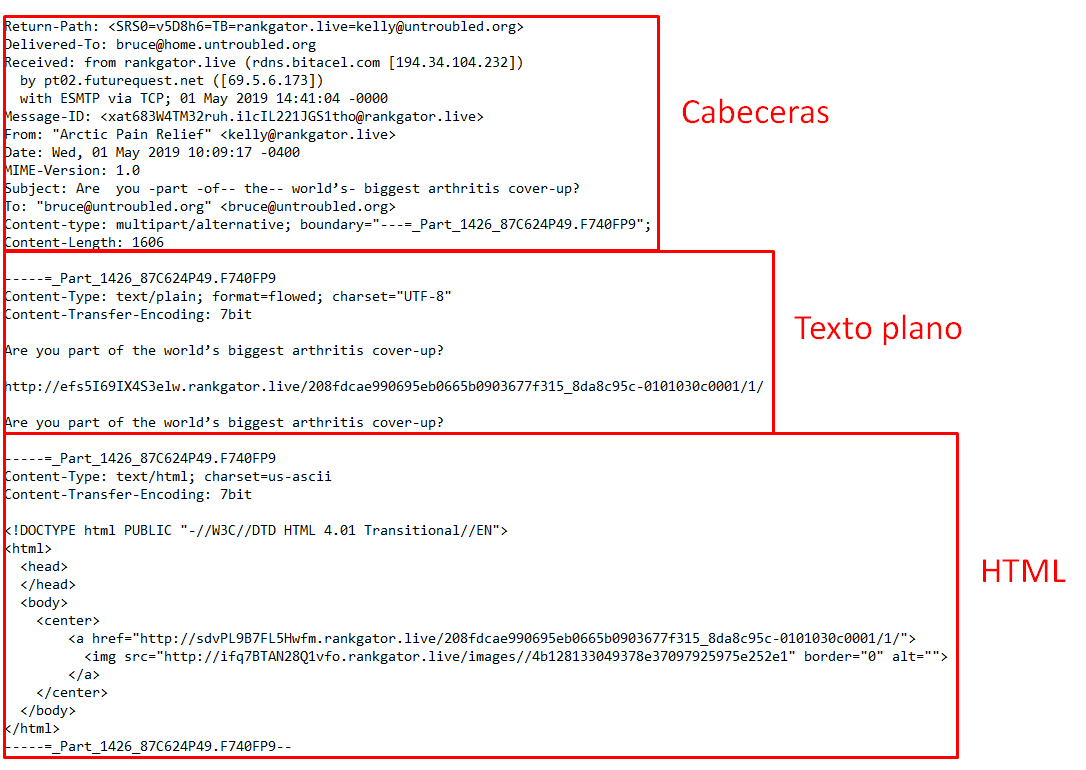
\includegraphics[scale=0.45]{imagenes/eml_example.png}
\caption{Ejemplo de EML}
\end{figure}


\section{Patrones maliciosos comúnmente usados en el correo electrónico}
Hasta el momento únicamente se ha analizado qué tipo de información se va a analizar, qué formato tiene y qué limitaciones de codificación y/o tamaño tienen. 

Entender esto con claridad permite entender algunas de las técnicas usadas por los ciberdelincuentes para poder atacar a sus víctimas. 

A continuación, se van a exponer una serie de patrones, que, si bien no permiten saber con seguridad de que se trate de un ataque, sí que permiten al menos tener cierta sospecha de que el correo sea malicioso.

Para el desarrollo de esta sección se han consultado entre otros los siguientes artículos 

\begin{itemize}
    \item A Framework for Detection and Measurement of Phishing Attacks \cite{phishing1}
    \item PhishDef: URL Names Say It All \cite{phishing2}
    \item Learning to detect phishing emails \cite{phishing3}
\end{itemize}

\subsection{Patrones maliciosos en Dominios} \label{patrones_maliciosos}
\subsubsection{Usar una gran cantidad de subdominios}
Un patrón bien conocido es utilizar una gran cantidad de subdominios con el objetivo de camuflar en ellos el dominio principal. 

En este tipo de ataques, el dominio a suplantar suele estar escrito al principio, seguido de más subdominios, hasta llegar el domino principal. De esta manera se dificulta su identificación. 

Un ejemplo de este tipo podría ser: 

\begin{verbatim}
    http://www.ugr.es.custsupportref1007.dllconf.info/r1/vm/
\end{verbatim}

Como se puede observar, la URL anterior se hace pasar por el dominio “www.ugr.es”, sin embargo, su dominio principal es “dllconf.info”.

Para detectar este tipo de ataque se podrían identificar el número de puntos “.” que tiene un dominio, de modo que cuantos más tenga, mayor es la probabilidad de que sea malicioso.

\subsection{Patrones maliciosos en Enlaces}
\subsubsection{Usar como dominio una IP}
Este patrón consiste en despistar al usuario usando como dominio una dirección IP y escribiendo en la ruta el dominio a suplantar. De esta forma si el usuario lee la dirección, el único domino que verá como tal es el suplantado y por tanto le dará legitimidad a la página. 

Un ejemplo de este patrón es: 

\begin{verbatim}
    http://211.233.39.145/www.ugr.es/login.html 
\end{verbatim}

Observando la dirección anterior puede verse como el único dominio como tal que aparece es el de “www.ugr.es”, aunque realmente el host es la IP “211.233.39.145”.

Detectar este tipo de patrón podría consistir en analizar si la máquina un dominio o una dirección IP. En caso de ser una IP, se podría decir que es posiblemente maliciosa. 

\subsubsection{Embeber una URL en la ruta de otra URL}
Una variación del patrón anterior es, en vez de usar una dirección IP, usar un dominio, generalmente muy corto y añadir la dirección a suplantar en la ruta, al igual que en el caso anterior.

Un ejemplo de este caso sería: 

\begin{verbatim}
    http://fkDom.tl/www.ugr.es/login.html 
\end{verbatim}

Al hacer esto, un usuario que no tenga cuidado no se percatará de que el dominio realmente es “fkDom.tl” y no “www.ugr.es” como el hubiera esperado. 

Para detectar este tipo de ataque, se podría comprobar que, en la ruta de un enlace, no haya ninguna otra ruta y en caso e haberla, tanto el dominio como la dirección completa serían sospechosos de ser perniciosos. 

\subsection{Patrones en archivos HTML}
\subsubsection{Ofuscación de la URL original una etiqueta tipo a}
Uno de los métodos más comunes y simples consiste en hacer uso de la etiqueta \verb!<a>! de HTML mostrando al usuario un valor distinto al recurso enlazado realmente mediante el atributo “href” de dicha etiqueta. 

Este patrón puede darse con varios de los posibles recursos que pueden ser enlazados mediante esta etiqueta. La cantidad de recursos depende en gran medida del soporte que tenga navegador para cada uno de los distintos esquemas asociados a cada recurso.

Todos los esquemas disponibles y a qué tipo de recurso que enlazan, está definidos por el IANA \cite{Schemas_dispo}

De entre todos ellos destacan los siguientes, por tener soporte en todos los navegadores y ser los más utilizados.

\paragraph{HTTP/HTTPS}
Es el caso más habitual, en este caso en el campo de texto se muestra un enlace a una página que no se corresponde con la enlazada. 

Un ejemplo sería \verb|<a href="https://www.ujr.es/">www.ugr.es</a>|

Este método es especialmente útil cuando se trata de ataques dirigidos a usuarios de dispositivos móviles ya que, en ellos, o no se ve la dirección en la que están navegado o sólo se ve parcialmente, lo cual dificulta en gran medida percatarse de este ataque. 

\paragraph{MAILTO}
Permite enviar abrir la aplicación de correo por defecto y añadir directamente al destinatario.En este caso se podría mostrar al usuario un email distinto al que se envía el mensaje. 

Por ejemplo: \verb|<a href="mailto:support@ujr.es"> support@ugr.es</a>|

\paragraph{Solución}
Una posible forma de detectar esta amenaza es, en primer lugar, comprobar si el texto mostrado al usuario es un enlace y en caso de serlo, compararlo con el enlace escrito en el atributo href de la etiqueta \verb!<a>!. En caso de ser distinto, el enlace del atributo href sería podría ser un enlace malicioso. 

\subsubsection{Uso de JavaScript}
Cuando un correo electrónico se abre en el navegador y está en formato HTML, puede contener código JavaScript que se ejecute automáticamente al abrirse. Si bien esto es hago normal en la web, no suele serlo en un mensaje de correo, ya que su contenido suele ser estático. 

Este tipo de código siempre va asociado a una etiqueta ``\verb|<script>|\\\verb|</script>|'', por tanto, una forma sencilla de detectar este patrón es simplemente comprobar si esta etiqueta aparece o no en el mensaje. 

\section{Integraciones de terceros}
A lo largo de esta sección se va a hablar de algunos servicios de terceros que pueden complementar los análisis de la plataforma. 

Algunos de ellos están relacionados directamente con la ciberseguridad y ya han sido descritos anteriormente, otros son de propósito general, pero pueden aportar información interesante a la hora de analizar un correo sospechoso. 

Para cada servicio se especificará en qué casos será relevante, cómo podría usarse y qué información adicional podría aportar.

\subsection{Virus Total}
Permite analizar archivos, enlaces, dominios y direcciones IP por varias decenas de servicios especializados dando así una visión más completa. 

Podría utilizarse para analizar alguno de los tipos de datos anteriores, que salgan como sospechosos o de los que el usuario dude.

\subsection{Metadefender}\label{Metadefender}
Es muy similar a Virus Total y por tanto de podría utilizar como alternativa a este. 

\subsection{Have I been pwned}
Permite saber si un correo ha estado involucrado en una brecha de seguridad. 

Podría utilizarse para saber si por ejemplo la dirección de la que proviene el correo ha estado expuesta en alguna brecha de seguridad, pudiendo sospechar de ella en caso de haber estado involucrada. 

\subsection{Whois}
Da información sobre un dominio o una dirección IP, como cuándo se registró o a quién pertenece.

Se puede utilizar para obtener más información sobre dominios sospechosos. También se puede utilizar para intentar descubrir a un ciberdelincuente. 

\section{Elección de la base de datos}
Debido a la gran cantidad de información que se va a manejar y al uso que se le va a dar a la base de datos, es el punto más importante que analizar, ya que una vez que se tenga una gran cantidad de datos almacenada, cambiar de sistema puede ser realmente complicado o simplemente imposible. 

La elección de un sistema de gestión de información que permita tanto insertar como hacer búsquedas rápidas en algo fundamental y de lo que va a depender el éxito o el fracaso del proyecto.

Tradicionalmente la información se guardaba en bases de datos relacionales interactuando con ellas mediante SQL. Esto ha hecho que en la actualidad haya multitud de gestores de bases de datos relacionales como MySQL\cite{MySQL}, MariaDB\cite{MariaDB}, SQLite\cite{SQLite}, PostgreSQL\cite{PostgreSQL} u Oracle\cite{Oracle} entre otros. Todos comparten el mismo lenguaje (SQL) para poder interactuar con ellos, aunque con pequeñas diferencias significativas, lo que hace que con algunos cambios se pueda cambiar de un sistema de gestión a otro y esto supone una gran ventaja.

Por otro lado, y aunque con menos uso, también existen muchos otros tipos de gestores de base de datos, que o bien no usan en absoluto el lenguaje SQL, como bien podría ser el caso de Mongo DB\cite{MongoDB}, o bien, además de usar SQL tienen ciertas peculiaridades que hacen que no sean únicamente una base de datos relacional. 

A diferencia de los sistemas relacionales, migrar de uno a otro, o incluso a uno relacional, suele suponer un gran cambio, no sólo a nivel de código, también a nivel conceptual y por tanto de diseño, por lo que elegir un sistema NoSQL, debe ser una elección meditada y analizada en detalle, ya que todos estos sistemas de almacenamiento suelen estar diseñados para tareas muy concretas y bien definidas, lo que hace que tengan ventajas e inconvenientes que hay que tener muy en cuenta.

Independientemente del sistema que se elija, se deben tener en cuenta los siguientes puntos:

\begin{itemize}
    \item Soportado o no por Azure
    \item Velocidad de las búsquedas
    \item Conocimientos previos
    \item Documentación
    \item Librerías disponibles 
    \item Facilidad para hacer relaciones entre datos
    \item Escalabilidad
\end{itemize}

\subsection{Sistemas relacionales SQL}

Son los sistemas más utilizados en la actualidad. Todos utilizan un lenguaje común para interactuar con ellos llamado lenguaje de consulta estructurada (Del inglés Structured Query Language, o SQL), aunque puede haber pequeñas diferencias entre ellos. 

Permite el uso del álgebra y el cálculo relacional para interactuar con el gestor de la base de datos, permitiendo de esta forma, buscar, modificar, añadir y eliminar información. 

Son usadas en multitud de proyectos de distinta envergadura por lo que su eficacia está muy probada, además de tener una amplia comunidad, una gran documentación y multitud de librerías para los distintos lenguajes de programación, algunas de ellas integradas dentro del propio lenguaje. 

\subsubsection{Ventajas}
\begin{itemize}
    \item Facilidad para cambiar de un gestor a otro (MariaDB, MySQL, SqLite, Oragle, Postgre SQL)
    \item Mucha documentación
    \item Una gran comunidad
    \item Conocimientos previos
    \item Una gran cantidad de librerías para multitud de lenguajes de programación
    \item Hacer relaciones entre es sencillo
    \item Búsquedas relativamente rápidas
    \item Respeta ACID
\end{itemize}

\subsubsection{Desventajas}
\begin{itemize}
    \item Inserciones lentas
    \item Escalado más complicado
    \item Esquema mucho más estricto
    \item Programación más lenta \footnote{El tener conocimientos previos unido a la gran comunidad, pueden mitigar este problema.}
\end{itemize}

\subsubsection{Conclusiones}

Usar un sistema de gestión de contenido relacional aporta una gran cantidad de ventajas, la mayor de ellas puede ser la velocidad de sus búsquedas, así como la facilidad para crear relaciones entre elementos. También es muy interesante que se pueda cambiar de un sistema a otro con relativa facilidad, en caso de que en el futuro uno de ellos cuente con ventajas adicionales sobre los demás. 

A todo esto, hay que sumarle que al ser un sistema con una larga trayectoria cuenta con una gran documentación, una comunidad amplia, multitud de librerías para la mayoría de los lenguajes de programación modernos y además se ha estudiado durante la carrera.
Los dos mayores problemas son por un lado la escalabilid
ad, que, aunque posible, es complicada. Esto puede suplirse al usar servicios en la nube que escalan de manera transparente los recursos de la base de datos para mantener las prestaciones, de ahí la importancia de usar un sistema soportado por Azure. 

El segundo problema es la lentitud de las inserciones, pero dado que los correos únicamente se van a insertar una única vez y que van a prevalecer las búsquedas sobre las inserciones, hace que, aunque este problema se deba tener en cuenta, no sea crítico siempre que el tiempo de inserción no se vuelva dramáticamente lento, en cuyo caso habría que escalar el sistema con la dificultad y el coste que esto supondría.

\subsection{Mongo DB}
Es un sistema gestor de bases de datos orientado a documentos, en vez de a tablas, y por tanto NoSQL. Concretamente este sistema de almacenamiento utiliza documentos en formato JSON, que se almacenan en formato BSON del término JSON binario y como lenguaje de consulta utiliza JavaScript.

Al no ser un sistema estructurado, los documentos pueden ser distintos y no tener una estructura fija definida. 

Su escalado horizontal es muy sencillo lo que asegura una gran disponibilidad y que no sea costoso. 
\subsubsection{Ventajas}
\begin{itemize}
    \item Escalado horizontal y vertical: En Mongo escalar tanto horizontal como verticalmente es algo simple que no requiere prácticamente de configuración. 
    \item Alta disponibilidad: que el escalado horizontal sea simple permite a Mongo tener una disponibilidad muy alta, ya que esta estructura permite una mejor respuesta a fallos eventuales del sistema. 
    \item Es muy rápido en las inserciones y en las actualizaciones de datos. 
    \item Tiene muchas más opciones para tratar datos de manera nativa. 
\end{itemize}

\subsubsection{Desventajas}
\begin{itemize}
    \item Las búsquedas son muy lentas.
    \item No hay posibilidad nativa de hacer uniones entre colecciones. 
    \item No respeta el modelo ACID.
\end{itemize}

\subsubsection{Conclusiones}
Que Mongo esté orientado a documentos hace que sea un gestor ideal para esta aplicación ya que lo que se va a guardar mayoritariamente son mensajes, es decir, documentos. 

Además, su tiene una gran velocidad de inserción, un escalado horizontal prácticamente nativo, y que los documentos no tengan una estructura fija por lo que se pueden personalizar de modo que se minimicen las búsquedas, hacen de Mongo una opción a tener muy en cuenta. 

También posee una gran cantidad de librerías para multitud de lenguajes de programación, una documentación muy completa y aunque no cuenta con la misma comunidad que los sistemas estructurados, sí que es bastante amplia por lo que no es complicado encontrar ayuda por parte de otros usuarios. 

Sin embargo, Mongo también presenta problemas importantes como sus búsquedas lentas, el hecho de tener que mantener la integridad de los datos de manera manual o la imposibilidad de hacer uniones entre datos de manera sencilla y rápida. Y es que, como se ha comentado anteriormente las búsquedas prevalecen sobre las inserciones, además hay una gran cantidad de relaciones que serían complicadas de mantener.
Otro punto débil es que, la posibilidad de migrar a otro sistema supondría el tener que comenzar desde cero, puesto que no hay ningún sistema compatible o similar. 

\subsection{Apache Cassandra}
Es un sistema de almacenamiento de datos que destaca por su escalado horizontal al ser una base de datos distribuida de escalado lineal, lo que es muy interesante ya permite predecir el número de nodos que se van a necesitar en función del número de peticiones que se tengan y las peticiones que es capaz de atender un único nodo. Esto quiere decir, que, si con un único nodo se pueden atender 1000 consultas por segundo, con dos se podrán atender 2000 y así sucesivamente \cite{Apache_Cassandra}. 

Su modelo de datos está basado en filas de columnas de clave-valor. 
\subsection{Ventajas}
\begin{itemize}
    \item Escalado horizontal y lineal.
    \item Velocidad de acceso.
\end{itemize}
\subsubsection{Desventajas}
\begin{itemize}
    \item Las relaciones entre elementos son complicadas.
    \item Es un cambio de paradigma complicado.
    \item La documentación no está acabada \cite{Apache_Cassandra_docu}.
    \item No se tienen conocimientos previos.
\end{itemize}
\subsubsection{Conclusión}
Lo más interesante de Cassandra es sin duda su escalado horizontal de manera lineal, sin embargo, cuenta con numerosos problemas como que la documentación no está totalmente acabada, que el modelo de estructura de datos no encaja con los modelos de datos de este proyecto, su comunidad de usuarios tampoco es muy amplia y tampoco se tienen conocimientos anteriores, por lo que la curva de aprendizaje puede suponer un gran problema. 

\subsection{Elasticsearch}
Elasticsearch\cite{Elasticsearch} no es tanto una base de datos como tal, es un motor de búsqueda y dado que lo que se van a almacenar son correos electrónicos, y por tanto, texto, puede ser muy buena opción, tal vez no como sistema de almacenamiento principal, pero sí como sistema complementario con el que realizar búsquedas avanzadas dentro de los propios mensajes. 

\subsubsection{Ventajas}
\begin{itemize}
    \item Escalado horizontal.
    \item Distribuido.
    \item Velocidad de búsqueda (incluso con búsquedas complejas).
    \item Se pueden aplicar algoritmos sobre las búsquedas.
    \item Se pueden usar analizadores de texto.
    \item Preparado para la inteligencia artificial \cite{Elasticsearch_IA}.
    \item La documentación está muy bien detallada \cite{Elasticsearch_docu}.
\end{itemize}
\subsubsection{Desventajas}
\begin{itemize}
    \item Velocidad de indexación.
    \item Su función principal es buscar texto, no almacenar información.
\end{itemize}
\subsubsection{Conclusión}
Aunque ElasticSearch es una herramienta muy atractiva y puede resultar muy útil en lo referente a búsquedas avanzadas de mensajes, no es viable usarla como sistema principal de almacenamiento ya que no es para lo que está pensada. 

De todas formas, podría ser muy interesante integrar esta herramienta en el servicio ya que ofrece funcionalidades muy interesantes y abre la posibilidad al uso de algoritmos de inteligencia artificial, lo que resulta especialmente interesante en mensajes de estafas, o de extorsión, en los que analizar detalles como enlaces, o dominios no es efectivo. 
\subsection{Conclusión}
Después de analizar múltiples motores de bases de datos, los que más se ajustan a las necesidades de este proyecto son o un sistema SQL o Mongo, sin estar realmente claro cuál puede funcionar mejor. 

Sin embargo, teniendo en cuenta que se van a realizar una gran cantidad de consultas y que éstas en Mongo son lentas, y que con la gran cantidad de relaciones que hay un sistema relacional ofrece un gran soporte, finalmente se va a optar por diseñar un sistema relacional.

Además, y aunque en un principio el desarrollo puede ser más lento, al tener experiencia previa en este tipo de sistemas, contar con una gran cantidad de documentación y una comunidad amplia en caso de tener algún problema eventual hará que el desarrollo no sea tan lento como lo pudiera ser si se tuvieran conocimientos previos de Mongo. 


\section{Diseño de la base de datos para un sistema relacional}
A la hora de realizar el diseño de la base de datos, se va a optar por hacer un diagrama entidad relación y además se va a explicar cada una de las tablas, aunque hay tablas intermedias o con una finalidad común que se describirán de manera genérica para facilitar la comprensión del documento. 

Aunque un esquema de este tipo está pensado para un sistema relacional, entender la estructura de este para pasarlo a otro tipo de diagrama y así adaptado a Mongo, la otra opción que se ha aproximado más a la solución no debería ser excesivamente complejo, más allá de adaptar las tablas a las colecciones de Mongo, integrar parte de las tablas intermedias en una única estructura y crear ciertos índices que faciliten las búsquedas.

En cambio, en lo que respecta al contenido, habría que reanalizar todo pues no habría ninguna forma sencilla de pasar el contenido de un sistema a otro. 

\subsection{Tablas}
Antes de analizar cada una de las tablas, se va a precisar algunos campos comunes entre tablas, así como algunas tablas comunes a algunos elementos. 
\subsubsection{Elementos comunes a varias tablas.}
%\renewcommand\labelitemii{$\square$}
\begin{itemize}
    \item[] 
    \begin{itemize}
        \item \texttt{Id}: Es la clave primaria de la tabla. Siempre es un entero. Se ha elegido esta opción por rendimiento. 
        \item \texttt{Ocurrences}: Es el número de veces que este elemento ha llegado para analizarse.
        \item \texttt{Score}: Es el valor de maliciosidad dado al elemento. Un número negativo indicará que es malicioso, un número positivo que es legítimo y cero que no se tiene información sobre dicho elemento. 
        \item \texttt{Hash}: Es un hash del elemento. Esto evita analizar dos veces un mismo elemento ahorrando tiempo de computación.  
        \item \texttt{Value}: Es el valor del propio elemento en sí.
        \item \texttt{Type}: Es una clave externa a un id de la tabla \verb!<Nombre Elemento>Type!, que identifica el tipo de elemento que es. 
        
        En algunos elementos se indican posibles tipos, esto se hace para facilitar la comprensión del documento, pero realmente se almacenan en la tabla \verb!<Nombre Elemento>Type!.
    \end{itemize}
\end{itemize}

\subsubsection{Tablas genéricas} \label{tablas_genericas}
\begin{itemize}
    \item \texttt{<Nombre Elemento>Delete}: Estas tablas están asociadas a cada uno de los elementos a almacenar susceptibles de ser borrados, como mensajes, emails,…
    
    Esto permite cumplir con el derecho al olvido de la ley de protección de datos europea.
    \begin{itemize}
        \item \texttt{Id}
        \item \texttt{Id<Nombre Elemento>}: es una clave externa al elemento en cuestión.
        \item \texttt{Hash}: Este hash permite identificar a cada elemento insertado, de modo que se le da al usuario la posibilidad de borrarlo si tiene el hash. 
        Está formado por el valor del elemento, una marca de tiempo y un valor aleatorio.
        Si dos usuarios introducen el mismo elemento, y sólo uno de ellos quiere borrarlo, el elemento permanecerá hasta que todos los usuarios que lo han introducido quieran borrarlo.
    \end{itemize}
        \item \texttt{<Nombre Elemento>Souces}: Identifica todas las fuentes de las que proviene el mensaje, pudiendo darle más o menos valor a la información que contenga en función de la fuente de la que provenga. Ej: emails identificados como maliciosos a mano tendrán más valor que los identificados por la IA (O al revés)
        \begin{itemize}
            \item \texttt{Id}
            \item \texttt{SourceName}: Nombre de la fuente de la que proviene.
            \item \texttt{Score}
        \end{itemize}
    \item \texttt{<Nombre Elemento>Souces}: Identifica todas las fuentes de las que proviene el mensaje, pudiendo darle más o menos valor a la información que contenga en función de la fuente de la que provenga. Ej: emails identificados como maliciosos a mano tendrán más valor que los identificados por la IA (O al revés)
    \begin{itemize}
        \item \texttt{Id}
        \item \texttt{Value}: Nombre de la fuente de la que proviene.
        \item \texttt{Score} 
    \end{itemize}
    \item \texttt{<Nombre Elemento>Type}: Identifica los posibles tipos del elemento, por ejemplo, si el elemento en cuestión es una criptomoneda, identifica el tipo de criptomoneda que es. 
    \begin{itemize}
        \item \texttt{Id}
        \item \texttt{Value}: Es el nombre del tipo.
    \end{itemize}
    \item \texttt{<Nombre Elemento>MaliciousChecks}: Identifica cada uno de los posibles patrones maliciosos de dicho elemento, como por ejemplo en el caso de una URL, no coincida el valor del atributo “href” con lo mostrado al usuario.
    \begin{itemize}
        \item \texttt{Id}
        \item \texttt{Value}: es el nombre de patrón.
        \item \texttt{Score}
    \end{itemize}
    \item \texttt{<Nombre Elemento1>\_<Nombre Elemento2>}: Esto son tablas intermedias para dejar la base de datos en Forma normal de Boyce-Codd cuando la multiplicidad es de muchos a muchos.
    \begin{itemize}
        \item \texttt{Id}
        \item \texttt{Id<Nombre Elemento1>}: es una clave externa a un id de la tabla \texttt{<Nombre Elemento1>}
        \item \texttt{Id<Nombre Elemento2>}: es una clave externa a un id de la tabla \texttt{<Nombre Elemento2>}
        \item \texttt{Date} \emph{(Opcional)}: Permite registrar el mismo elemento, mediante la misma fuente, más de una vez. Esto puede permitir detectar elementos muy analizados en un instante de tiempo, típico por ejemplo cuando se realiza una nueva campaña de phishing, dicho elemento tendrá un pico de análisis cuando se realice la campaña.
    \end{itemize}
\end{itemize}

\subsubsection{Tablas específicas de cada elemento}
Son cada uno de los elementos que se van a guardar en la base de datos.

Se pueden distinguir tres tipos de datos: 

\begin{enumerate}
    \item Los mensajes en sí. Es la tabla principal del proyecto y con la que están relacionada la mayoría de las tablas principales.
    \item Los elementos que se detectan de cada mensaje. Por ejemplo: direcciones de emails, dominios, links, …
    \item Los distintos tipos de mensajes que hay, por ejemplo, mensajes de correo electrónico (Los elementos principales), mensajes de Whatsapp o Telegram, SMS, mensajes de redes sociales como Instagram, Facebook o Twitter, …
    Estas tablas siempre tendrán una clave externa a la tabla Message, lo que permite identificar un mismo texto mediante distintos tipos de mensaje. Por ejemplo una campaña de phishing 
    \item Se podrían distinguir un cuanto tipo de elementos que son todas las tablas auxiliares específicas de elementos concretos y no detalladas anteriormente. Este tipo de tablas son, por ejemplo, la tabla de países de los números de teléfono, la de las cabeceras de los emails, … Son tablas que añaden detalles o facilitan la implementación. 
    
\end{enumerate}

\paragraph{Mensajes}
\begin{itemize}
    \item \texttt{Message}: es la tabla principal del proyecto. En esta tabla se guardarán los mensajes o la ubicación de estos y está formada por los siguientes campos: 
\begin{itemize}
    \item \texttt{Id}
    \item \texttt{Hash}
    \item \texttt{Value}
    \item \texttt{Occurrences}
    \item \texttt{Score}
    \item \texttt{Kind}: [eml, html, text]
    \item \texttt{AnalyzedBy}: en caso de tener varios lenguajes o varias formas de análisis, permite saber con qué lenguaje se ha hecho
    \item \texttt{Status}: indica si está analizado o pendiente de analizar.
    \item \texttt{AnalyzedAt}: indica la fecha del último análisis. (Esto permite que si en el futuro se añade nuevos análisis, sólo se analicen los archivos anteriores a la fecha de implementación)
\end{itemize}
\end{itemize}
\paragraph{Elementos a detectar en los mensajes}
\begin{itemize}
    \item \texttt{IpAddresss}: Son direcciones ip que pueden ser maliciosas o no, en función del score.: 
\begin{itemize}
    \item \texttt{Id}
    \item \texttt{Hash}
    \item \texttt{Value}
    \item \texttt{Occurrences}
    \item \texttt{Score}
    \item \texttt{ipV4}: indica si la ip es v4 o v6.
\end{itemize}
\item \texttt{Domain}: en esta tabla se almacenan tanto dominios como subdominios. Los subdominios tendrán una clave externa al dominio. 

Puede haber dominios en los que todos sus subdominios sean maliciosos o en los que no tengan relación. (Véase el caso de los subdominios de wordpress.com o blogspot.com)

Esta tabla está relacionada con la tabla ipAddress, anteriormente detallada permitiendo tanto a un dominio tener varias direcciones IP y como tener varios dominios apuntando a la misma IP, y estas ser tanto IPv4 como IPv6

\begin{itemize}
    \item \texttt{Id}
    \item \texttt{Hash}
    \item \texttt{Value}
    \item \texttt{Occurrences}
    \item \texttt{Score}
    \item \texttt{DomainId}: permite identificar el domino en caso de ser un subdominio.
\end{itemize}
\item \texttt{URL}: Son enlaces, es decir una ruta de un dominio y van a estar siempre asociadas a él. Este es un elemento clave a analizar pues la inmensa mayoría de los ataques de phishing se producen al ingresar en una url falsa.
\begin{itemize}
    \item \texttt{Id}
    \item \texttt{Hash}
    \item \texttt{Value}
    \item \texttt{Occurrences}
    \item \texttt{Score}
    \item \texttt{Domain}: Es un clave externa a la tabla domains como ya se ha detallado con anterioridad.
\end{itemize}
\item \texttt{EmailAddresses}: En esta tabla se almacenarán todas las direcciones de correo electrónico que se detecten. 

Esta tabla también tiene especial relevancia porque la mayoría de los ataques se realizan por correo electrónico. Esta tabla se relaciona con la tabla domain, anteriormente detallada. Además, también se tiene en cuenta el enmascaramiento de direcciones falsas mediante el tag “\verb!<a>!” y el atributo “href” de html.
\begin{itemize}
    \item \texttt{Id}
    \item \texttt{Hash}
    \item \texttt{Value}
    \item \texttt{Occurrences}
    \item \texttt{Score}
    \item \texttt{Domain}: Es un clave externa a la tabla domains como ya se ha detallado con anterioridad.
\end{itemize}

\end{itemize}
*La implementación permite añadir nuevos elementos a detectar, tales como cuentas bancarias, o principales palabras.

\section{Elección del lenguaje de programación}
El lenguaje de programación es el punto de unión entre la base de datos y la interacción del usuario. Se distinguen dos partes, por un lado, la parte de análisis del mensaje, extracción de datos e inserción de estos en la base de datos y, por otro lado, la visualización.

Lo ideal sería utilizar el mismo mensaje para ambos propósitos ya que daría homogeneidad al proyecto, aunque esto supone que la búsqueda de un lenguaje que satisfaga todos los requisitos sea más compleja.

Independiente a esto, se va a dar prioridad a lenguajes soportados por el servicio de Azure Functions ya que permite escalar el servicio de manera transparente y el costo va ligado a la utilización del servicio evitando tener costes iniciales o fijos.

De esta manera, los lenguajes candidatos serían C\#, F\#, Node.js, Python, Java o PHP \footnote{PHP ya no está disponible, pero al comienzo de este trabajo sí lo estaba.}.

Dentro de los lenguajes anteriores, se van a valorar: 
\begin{description}
    \item [Java:] por el conocimiento previo, por su portabilidad, por tu soporte con multitud de tipos de bases de datos y por la cantidad de librerías existentes para este lenguaje.
    \item [Python:] por ser uno de los lenguajes de programación más usados en Big Data y en inteligencia artificial, por la sencillez del lenguaje, y por tener soporte para web.
    \item [Node.js:] por su uso en la web, por tu portabilidad y por su soporte completo de expresiones regulares.
    \item [PHP:] por ser run estándar en la web, por su soporte completo a expresiones regulares, por su fácil integración con múltiples sistemas de bases de datos. 
\end{description}

Se van a valorar los siguientes aspectos:
\begin{enumerate}
    \item Librerías para bases de base de datos SQL\footnote{Adicionalmente y por si finalmente se migra a Mongo, se comprobará si existe o no algún tipo de soporte para este tipo de base de datos.}
    \item Soporte y rendimiento con expresiones regulares.
    \item Librerías para analizar archivos EML.
    \item Librerías para archivos HTML. 
    \item Funciones hash, en concreto SHA1.
    \item Soportado o no por Azure.
    \item Facilidad para crear una web mediante dicho lenguaje.
    \item Documentación.
    \item Comunidad.
\end{enumerate}

\subsection{Java}
Java es un lenguaje multidispositivo, con una gran comunidad, una documentación muy completa y tiene una gran cantidad de librerías para todo tipo de bases de datos. 
\subsubsection{Soporte para bases de datos}
Java cuenta con una librería nativa para conectarse a bases de datos relacionales conocido como Java Database Connectivity [JDBC] \cite{JDBC_oracle} que cuenta con controladores para multitud de bases de datos relacionales como Postgresql \cite{JDBC_postgresql}, MySQL \cite{JDBC_MySQL} o MariaDB \cite{JDBC_MariaDB}

También cabe mencionar que hay ORM’s que facilitan la tarea de acceder a la base de datos, el más famoso puede ser Hibernate \cite{Hibernate}, además, este mismo ORM ofrece soporte para Mongo. 

\subsubsection{Soporte para expresiones regulares}
Java tiene la clase Pattern \cite{java_Pattern_class} a partir de su versión 7 la cual permite trabajar de manera nativa con expresiones regulares. 

\subsubsection{Librerías para analizar archivos EML}
La mejor forma de leer archivos EML en Java es haciendo uso de la librería JavaMail \cite{JavaMail}. Esta es una librería opcional en Java SE y está incluida en Java EE por lo que tiene soporte por parte de Oracle \cite{java_JavaMail}.

\subsubsection{Librerías para archivos HTML}
Para leer archivos con formato HTML se puede usar la librería Jsoup \cite{jsoup}.

Otras librerías que también pueden ser interesantes para leer archivos de la familia XML puede ser Jerry \cite{jerry} con Lagarto \cite{jerry}.

\subsubsection{Funciones hash}
Los algoritmos de hash en Java se encuentran en la clase MessageDigest \cite{java_MessageDigest} y cuentan con al menos las funciones MD5, SHA-1 y SHA-256.

\subsubsection{Facilidad para crear una web mediante dicho lenguaje}
Lenguajes debido a la máquina virtual donde se ejecuta código, por eso se utilizar un servidor Tomcat \cite{tomcat}.

Encontrar hostings que soporten este tipo de servidores no es tan fácil como servidores que ejecuten código PHP.

Dentro de las librerías más famosas para crear una web con java están Spring \cite{Spring} y Structs \cite{Struts}. 

\subsubsection{Documentación}
Java posee una documentación muy detallada, además no es difícil encontrar una cantidad de ayuda y recursos en la web. \cite{java_docu}

\subsubsection{Conclusión}
Java es un lenguaje desarrollado por Oracle con una gran trayectoria, lo que hace que tenga una documentación muy buena, multitud de ejemplos en la web y una gran cantidad de librerías.

Además, es un lenguaje compilado lo que debería hacer que fuese rápido si no se ejecutase en una máquina virtual \cite{java_vm}, lo que hace que consuma muchos recursos, especialmente RAM. 

\subsection{Python}
Python es un lenguaje de muy alto nivel, que compila a código C.

Su rendimiento no es tan alto como otros lenguajes de bajo nivel, pero es sencillo de programar. 

\subsubsection{Soporte para bases de datos}

Actualmente Python posee varios conectores para distintos gestores de bases de datos relacionales como los ya mencionados, algunos de estos son Mysql \cite{python_mysql}, MariaDB que utiliza el mismo conector que MySQL \cite{python_mariadb}, o Postgresql \cite{python_Postgresql}.

En caso de migrar posteriormente a MongoDB, también posee el controlador Pymongo \cite{python_MongoDB}.

\subsubsection{Soporte para expresiones regulares}
Para el uso de expresiones regulares Python 3 cuenta con la librería re \cite{python_regex}.

\subsubsection{Librerías para analizar archivos EML}
Para analizar archivos con formato EML, se puede usar el paquete eml-parser \cite{python_eml_parser} o el paquete emaildata \cite{python_emaildata}.

\subsubsection{Librerías para archivos HTML}
Python 3 cuenta con un módulo llamado HTMLParser \cite{python_HTMLParser} destinado a leer archivos con formato HTML. 

\subsubsection{Funciones hash}
Las funciones hash están implementadas en el módulo hashlib \cite{python_hashlib} y tiene soporte para sha1, sha224, sha256, sha384, sha512, o md5 entre otras. 

\subsubsection{Facilidad para crear una web mediante dicho lenguaje}
Actualmente existen varios frameworks que permiten crear una web con Python, los más famosos son Django \cite{python_Django} y Flask \cite{python_Flask}.

\subsubsection{Documentación}
La documentación de Python se puede encontrar en su página oficial \cite{python_docu} y aunque se echa en falta algo más de claridad, no es difícil encontrar buenos ejemplos en internet. 

\subsubsection{Conclusión}
Python es un lenguaje que permite un desarrollo rápido, con una gran comunidad de usuarios y con gran cantidad de librerías. 
Sin embargo, su sintaxis es bastante distinta a la de los demás lenguajes, tampoco tiene un gran rendimiento y su documentación no es muy completa.

\subsection{Node}
\subsubsection{Soporte para bases de datos}
Node posee varios paquetes para conectarse a bases de datos SQL como el paquete mysql \cite{node_mysql}, o el paquete mysql2 \cite{node_mysql2}.

Por otro lado, en caso de querer usar una base de datos Mongo, tiene el paquete mongodb \cite{node_mongo_driver}, además cuenta con el ORM mongoosejs \cite{node_Mongoosejs}.

\subsubsection{Soporte para expresiones regulares}
Node tiene soporte nativo para expresiones regulares mediante la clase RegExp \cite{node_regex}.

\subsubsection{Librerías para analizar archivos EML}
Para leer un archivo EML con node se puede usar el paquete mailparser \cite{node_mailparser} o el paquete eml-format \cite{node_eml_format}.

\subsubsection{Librerías para archivos HTML}
Los archivos de la familia XML, entre ellos los  que tienen formato HTML, puede ser analizados con el paquete htmlparser2 \cite{node_htmlparser2}.

\subsubsection{Funciones hash}
Para utilizar funciones hash Node cuenta con el módulo Crypto \cite{node_Crypto}. La lista de algoritmos disponibles depende del módulo OpenSSL que tenga instalado el sistema operativo \cite{node_Crypto_algorithm_options} y se puede obtener de la siguiente forma: 
\begin{verbatim}
let crypto = require('crypto');
let listOfSupportedHashes = crypto.getHashes(); 
\end{verbatim}

\subsubsection{Facilidad para crear una web mediante dicho lenguaje}
Uno de los principales usos de Node es para la creación de webs, por lo que ofrece un amplio soporte para ello. Uno de los principales frameworks para este propósito es Expressjs \cite{node_expressjs}.

\subsubsection{Documentación}
La documentación de Node es muy completa y con varios ejemplos de uno dentro de la misma web \cite{node_docu}. 

\subsubsection{Conclusión}
Pese a ser un lenguaje interpretado tiene un rendimiento muy aceptable gracias al buen trabajo de Google con su motor de JavaScript V8 \cite{node_engine}, además gracias a su programación mediante callbacks y promesas hacen que sea especialmente interesante ya que se pueden realizar tareas en paralelo de manera sencilla.

Su documentación es excelente, aunque no tiene tantas librerías como los otros lenguajes.

Por otro lado, permite tener un único lenguaje de programación para todo el proyecto, tanto para la parte del análisis como para la parte de la web. 


\subsection{PHP}

\subsubsection{Soporte para bases de datos SQL}\label{php_bases_de_datos}
PHP ofrece soporte nativo para una gran cantidad de bases de datos relacionales mediante la clase PDO \cite{php_pdo}, como MySQL o PostgreSQL \cite{php_pdo_drivers}.

\subsubsection{Soporte para expresiones regulares}
Las expresiones regulares pueden usarse de manera nativa en PHP como demuestra su documentación \cite{php_pcre}.

\subsubsection{Librerías para analizar archivos EML}
Para poder leer los archivos con formato EML, se puede usar de manera nativa la familia de funciones mailparse \cite{php_Mailparse}. Para un soporte más completo se puede usar la librería php-mime-mail-parser \cite{php_php_mime_mail_parser}.

\subsubsection{Librerías para archivos HTML}
PHP tiene de forma nativa un conjunto de clases para tartar con archivos de la familia XML como sería el caso del formato HTML \cite{php_dom}.

\subsubsection{Funciones hash}
Este lenguaje soporta de manera nativa una gran cantidad de funciones hash de manera nativa \cite{php_hash}. 
Facilidad para crear una web mediante dicho lenguaje
PHP es uno de los lenguajes más utilizados para web, de hecho, es prácticamente el uso principal de este lenguaje, por lo que se ofrece de manera nativa una gran cantidad de facilidades para crear webs. 
Aunque también posee varios frameworks como Synfony \cite{php_Symfony} o Laravel \cite{php_laravel}.

\subsubsection{Documentación}
La documentación es muy completa, teniendo soporte incluso en español \cite{php_docu}. Además, gracias a su larga trayectoria se pueden encontrar de manera sencilla multitud de ejemplos prácticos para una gran cantidad de problemas. 

\subsubsection{Conclusión}
PHP es un lenguaje que está especialmente diseñado para web, tiene una gran trayectoria y aunque su rendimiento era bastante pobre, ha mejorado en gran medida en su versión 7.\cite{php_Benchmark}

De todos los lenguajes es el único que permitiría hacer el proyecto de manera prácticamente nativa, especialmente interesante es el uso de la clase PDO, que te permite cambiar de un gestor de base de datos a otro de manera practica mente transparente. 

Su documentación es aceptable, con ejemplos y la única disponible en español, también tiene una gran comunidad, lo que facilita encontrar ejemplos a problemas conocidos. 

\subsection{Rendimiento en expresiones regulares}
Se ha encontrado un benchmark \cite{regex_benchmark} totalmente independiente en el que se analiza el rendimiento con expresiones, además, con expresiones regulares similares a las usadas en este proyecto, de diferentes lenguajes de programación.  De todos los analizados, se va a extraer la información de los que conciernen a este proyecto. 

\begin{table}[htbp]
    \begin{center}
        \begin{tabular}{| m{2.8cm} || m{2cm} | m{2cm} | m{2cm} | m{2cm} |}
            \hline
            Language & Email (ms) & URI (ms) & IP (ms) & Total (ms) \\ 
            \hline \hline 
            PHP & 29.20 & 28.05 & 9.12 & 66.37\\
            Node.js & 81.87 & 67.16 & 2.04 & 151.07\\
            Python PyPy3 & 354.38 & 314.82 & 367.19 & 1036.39\\
            Java & 310.30 & 326.81 & 732.19 & 1369.30 \\
            \hline
        \end{tabular}
    \caption{Comparativa del rendimiento en la evaluación de expresiones }
    \label{table:regex_benchmark}
    \end{center}
\end{table}

Como puede verse en la tabla \ref{table:regex_benchmark}, el más rápido es PHP, a una distancia prudente está Node, muy por detrás quedan Python y Java. 
\subsection{Conclusión}
De todos los lenguajes analizados, los más interesantes son PHP y Node.

PHP destaca por tener de manera nativa prácticamente todo lo necesario para el desarrollo, por la facilidad para cambiar a otro tipo de base de datos relacional de manera prácticamente transparente y por su alto rendimiento.

En el otro lado, Node también tiene un buen rendimiento, existen todas librerías necesarias para este proyecto, su documentación es muy buena y permitiría tener un único lenguaje de programación para todo el desarrollo. 

\subsubsection{Resultado final}
Finalmente y comparando las ventajas e inconvenientes que nos ofrencen ambos lenguajes, se ha optado por elegir PHP ya que, por un lado prácticamente no es necesario instalar dependencias externas y por otro migrar de un gestor de base de datos de otro, siempre que sean relacionales como es el caso, es bastante sencillo.